\documentclass[11pt, oneside]{article}
\usepackage[margin=1in]{geometry}
\geometry{letterpaper}
\usepackage{graphicx}
\usepackage{amssymb}
\usepackage[parfill]{parskip}
\usepackage{amssymb}
\usepackage{amsmath}
\usepackage{listings}
\usepackage{color}
\usepackage{standalone}
\usepackage{gensymb}
\usepackage{tikz}
\usetikzlibrary{matrix,chains,positioning,decorations.pathreplacing,arrows}
\usepackage{wrapfig}
\usepackage{epstopdf}

\graphicspath{ {images/} }

\def\layersep{2.5cm}

\sloppy
\definecolor{lightgray}{gray}{0.5}
\setlength{\parindent}{0pt}
\definecolor{dkgreen}{rgb}{0,0.6,0}
\definecolor{gray}{rgb}{0.5,0.5,0.5}
\definecolor{mauve}{rgb}{0.58,0,0.82}

\lstset{frame=tb,
  language=Matlab,
  aboveskip=3mm,
  belowskip=3mm,
  showstringspaces=false,
  columns=flexible,
  basicstyle={\small\ttfamily},
  numbers=none,
  numberstyle=\tiny\color{gray},
  keywordstyle=\color{blue},
  commentstyle=\color{dkgreen},
  stringstyle=\color{mauve},
  breaklines=true,
  breakatwhitespace=true,
  tabsize=3
}

\title{Neuro 120 Homework 3: Vision and Deep Networks}
\author{William Schmitt and Will Drew}
\date{Due: Thursday 8 November 2018}

\begin{document}
\maketitle

\section{Question 1: Early Vision and Convolutions}

\subsection{Difference of Gaussians Filter}

We created the difference of Gaussians filter via the following line of code: \lstinline{dog = fspecial('gaussian', [51 51], 3) - fspecial('gaussian', [51 51], 7);} and plotted this with \lstinline{surf(dog)} to produce the following image in Figure \ref{fig:dog}.

\begin{figure}[ht!]
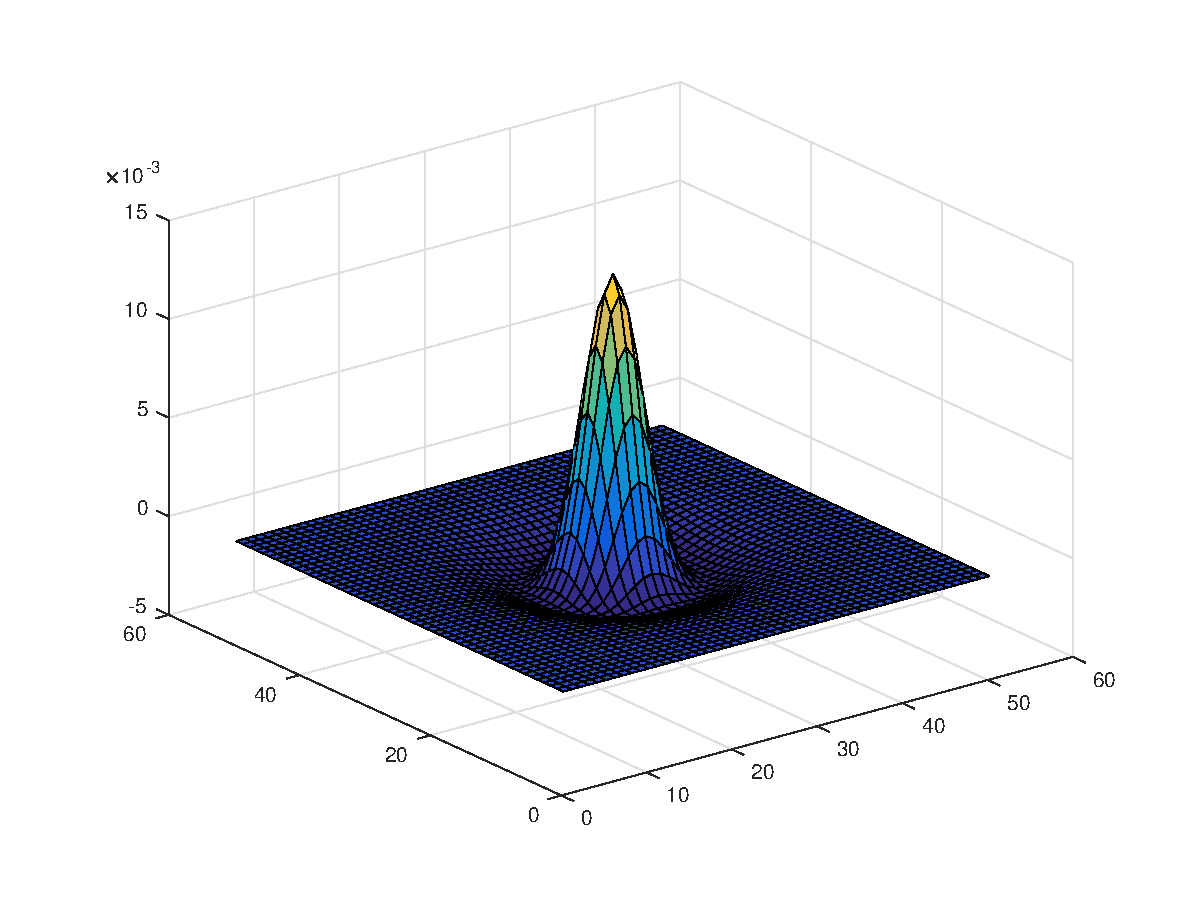
\includegraphics[width=1\textwidth]{dog.eps}
\caption{The coefficients of the difference of Gaussians filter.}
\label{fig:dog}
\end{figure}

\subsection{Mach band Convolution}

We convolve the Mach band image with the filter from part A via the following line of code: \lstinline{res = conv2(im_mach, dog, 'valid');}. We then plot this with the command, \lstinline{imagesc(res)}. This produces Figure \ref{fig:machConv}. We can see from this figure that the Mach band illusion results in activity at the boundary of the lines in the images (as seen by the one white line, corresponding to an increase in the RGC responses, and by the one black line, corresponding to a decrease in the RGC responses). Thus, these RGCs are detecting two ``edges'' in the Mach band illusion. This illusion is due to the center-surround nature of the difference of Gaussians filter the RGCs are modeled with.

\begin{figure}[ht!]
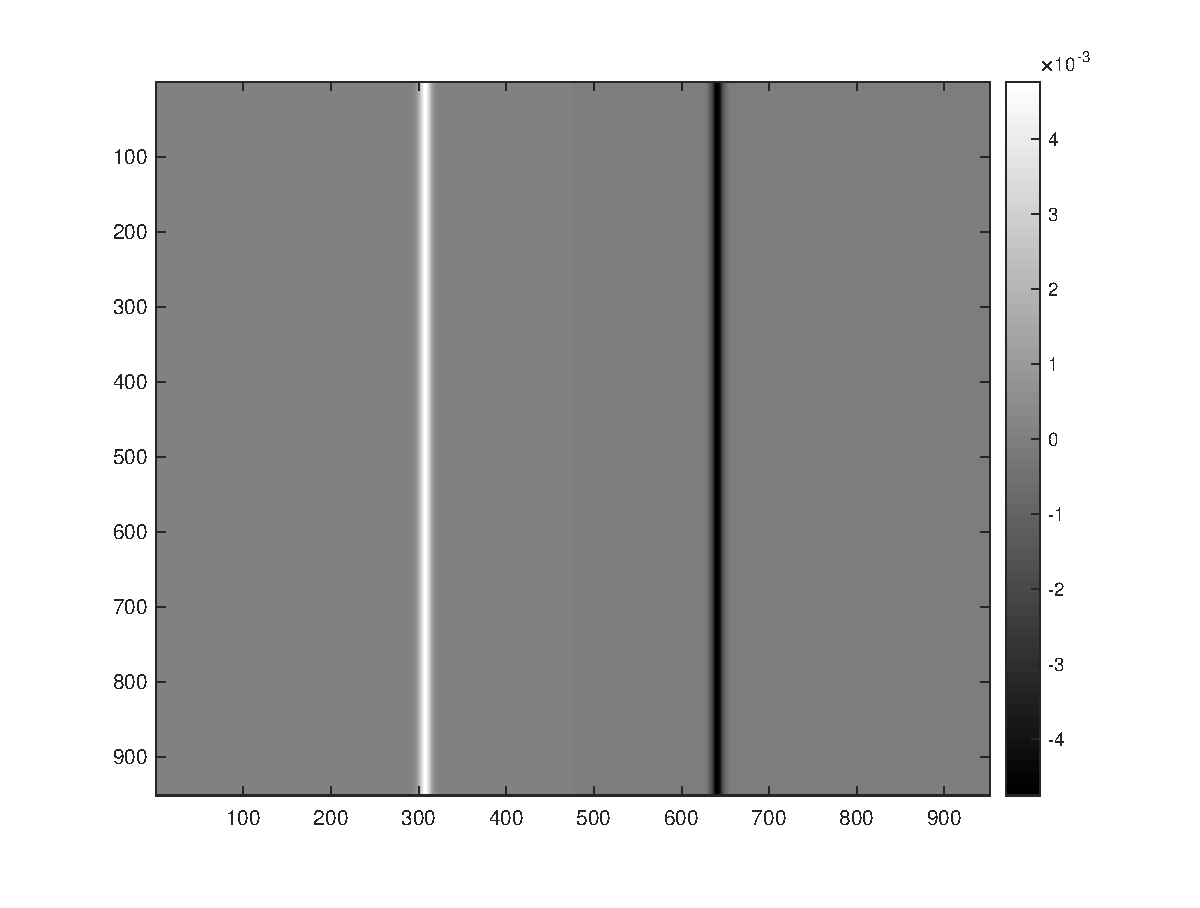
\includegraphics[width=1\textwidth]{mach_dog_conv.eps}
\caption{The result of convolving the Mach bands image with the filter from part A.}
\label{fig:machConv}
\end{figure}

\subsection{Mach band Convolution with a Small Constant}

We convolve the Mach band image with the filter from part A plus a small constant of $0.00001$ via the following line of code: \lstinline{dog2 = dog + 0.00001; res = conv2(im_mach, dog2, 'valid');}. We then plot this with the command, \lstinline{imagesc(res)}. This produces Figure \ref{fig:machConv2}. We can see from this command that again, the RGC model is detecting the two edges in the same locations. However, there is now a background gradient from light to dark (going left to right), with the increase (decrease) in activity being noticeably more at the first (second) edge. This relates to the Mach band illusion in that it is this detection of an edge in an image which has a larger overall gradient of brightness, which causes the person to perceive one side of the edge to be brighter than it actually is and one side to be darker than it actually is. 

\begin{figure}[ht!]
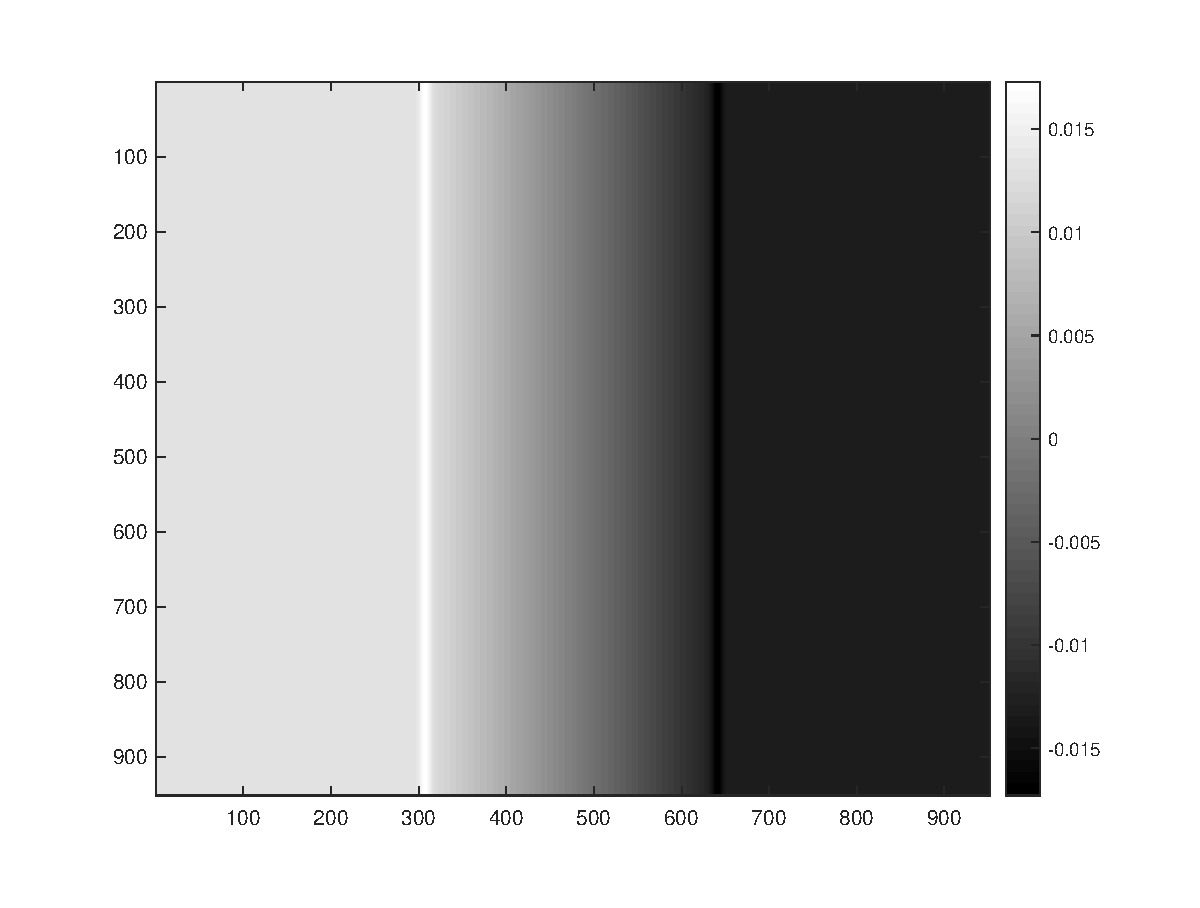
\includegraphics[width=1\textwidth]{mach_dog_conv2.eps}
\caption{The result of convolving the Mach bands image with the filter from part A plus a small constant.}
\label{fig:machConv2}
\end{figure}

\subsection{Checkerboard Illusion}

We convolve the checkerboard illusion with the filter from part A via the following of code: \lstinline{res = conv2(im_cb, dog, 'valid');}. We then plot this with the command, \lstinline{imagesc(res)}. This produces Figure \ref{fig:checkConv}. We can see from this figure that there are slight (barely noticeable) gray circles at the intersection of the lines compared to the middle of a stripe. Thus, we see that the center-surround nature of the RGCs produce a decreased response at the intersection of these stripes, which is why it appears to our eyes that there are gray circles at the intersections when they are really just white.

\begin{figure}[ht!]
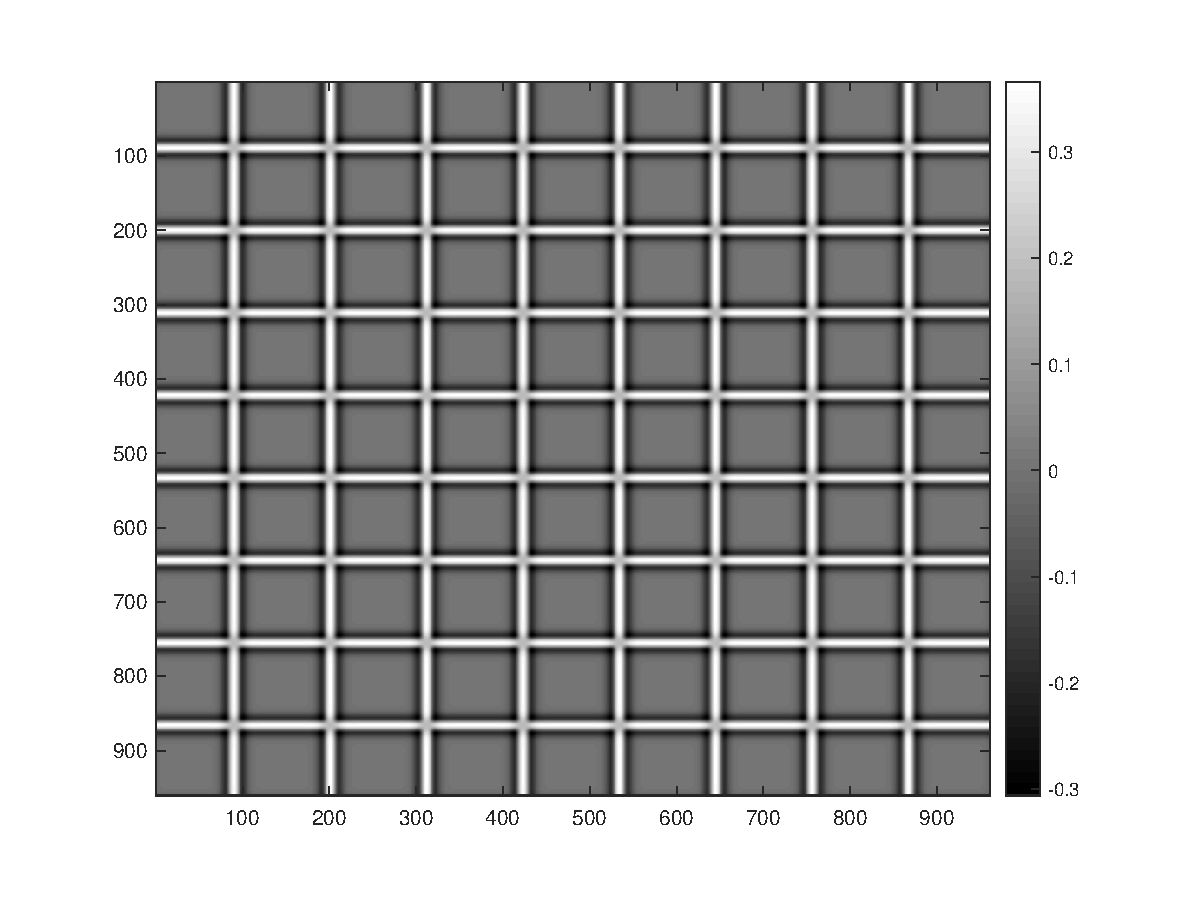
\includegraphics[width=1\textwidth]{check_dog_conv.eps}
\caption{The result of convolving the checkerboard illusion image with the filter from part A.}
\label{fig:checkConv}
\end{figure}

\subsection{Checkerboard Illusion with a Narrower Filter}

We make a new difference of Gaussians filter with the following code: \lstinline{dog3 = fspecial('gaussian', [51 51], 3) - fspecial('gaussian', [51 51], 7);}. We plotted this with \lstinline{surf(dog3)} to produce the following image in Figure \ref{fig:dog3}. We then convolve the checkerboard illusion with this filter via the following code: \lstinline{res = conv2(im_cb, dog3, 'valid');}. This produces Figure \ref{fig:checkConv2}. We can see from this figure that the intersections of the stripes are the same color as the stripes themselves, which explains why when we focus on a certain intersection, the gray circle appears to disappear. The RGCs in our fovea, which are modeled here, are not tricked by the illusion.

\begin{figure}[ht!]
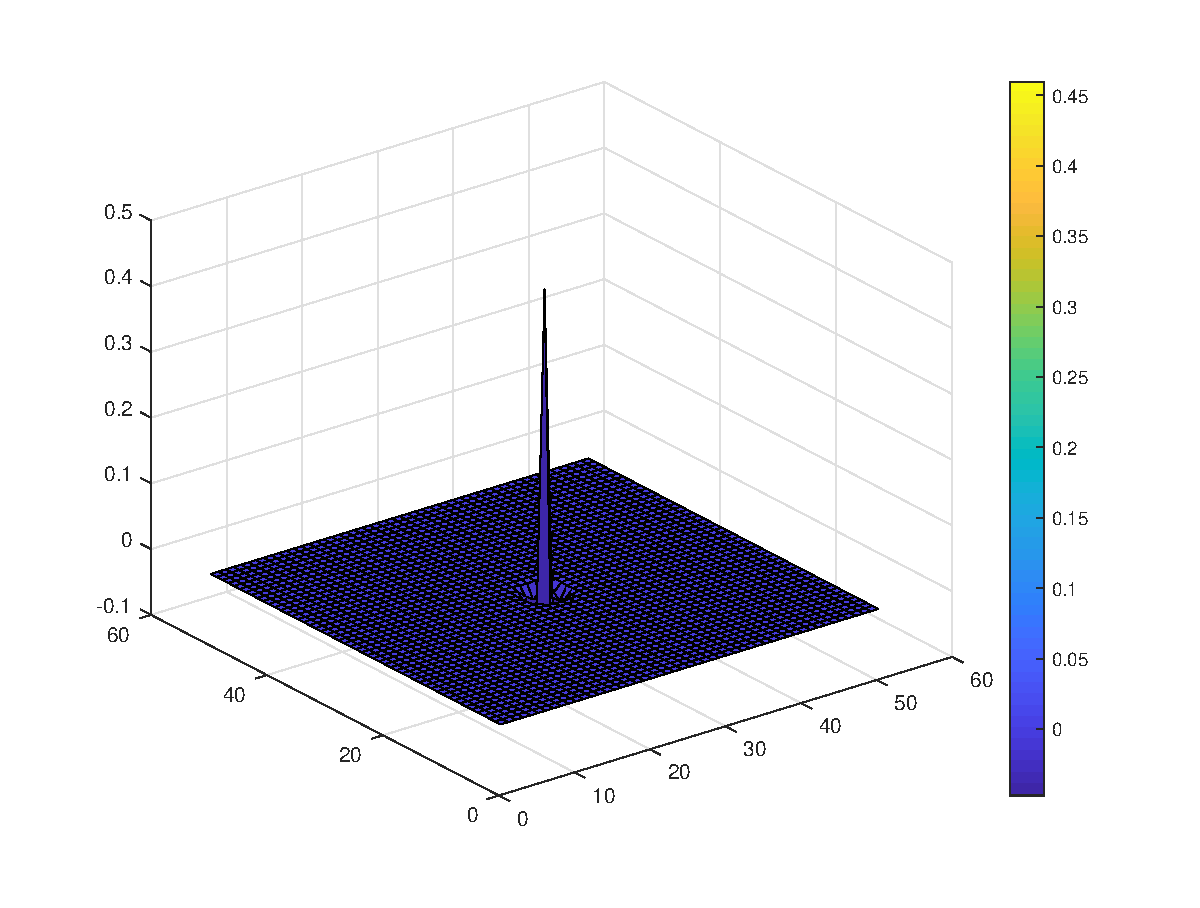
\includegraphics[width=1\textwidth]{dog3.eps}
\caption{The coefficients of a narrower difference of Gaussians filter.}
\label{fig:dog3}
\end{figure}

\begin{figure}[ht!]
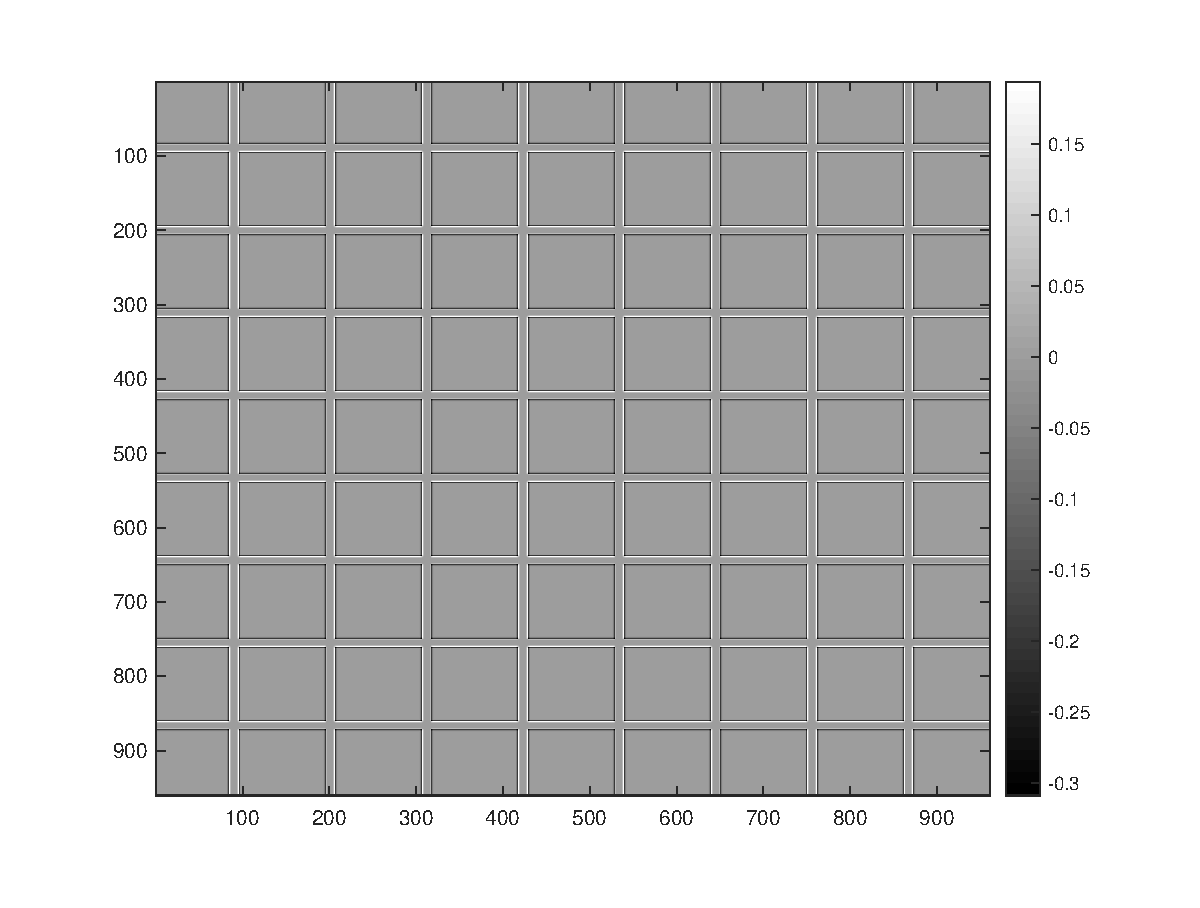
\includegraphics[width=1\textwidth]{check_dog3_conv.eps}
\caption{The result of convolving the checkerboard illusion image with a narrower filter.}
\label{fig:checkConv2}
\end{figure}

\subsection{Peppers}

We convolved the pepper image with both the filter from part A and that from part E via the following code:
\lstinputlisting[firstline=71, lastline=79]{earlyvision.m}.
This produces Figures \ref{fig:pepper_broad} and \ref{fig:pepper_narrow}. We can see from these figures that in the image convolved with the broader filter (from Part A), the gross gradient differences between the peppers is preserved. Further, one can distinguish (somewhat) some peppers from others, though the acuity of an individual pepper is low. However, with the narrower filter, the gradient information is lost (i.e. we can't tell which peppers are darker and which are lighter), but we can make out fine details on each pepper (i.e. the lines of the onion).

\begin{figure}[ht!]
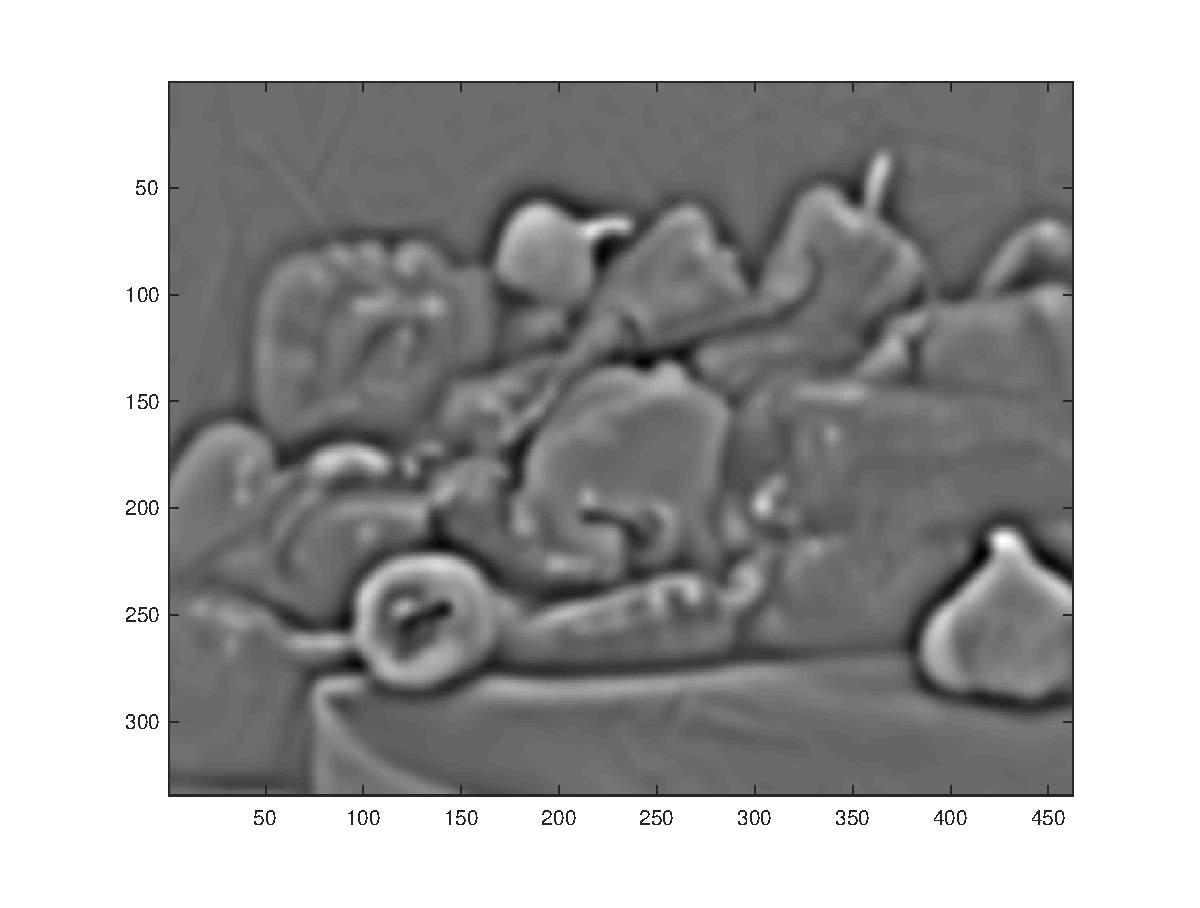
\includegraphics[width=1\textwidth]{peppers_dog_conv.eps}
\caption{The result of convolving the peppers image with the original filter from part A.}
\label{fig:pepper_broad}
\end{figure}

\begin{figure}[ht!]
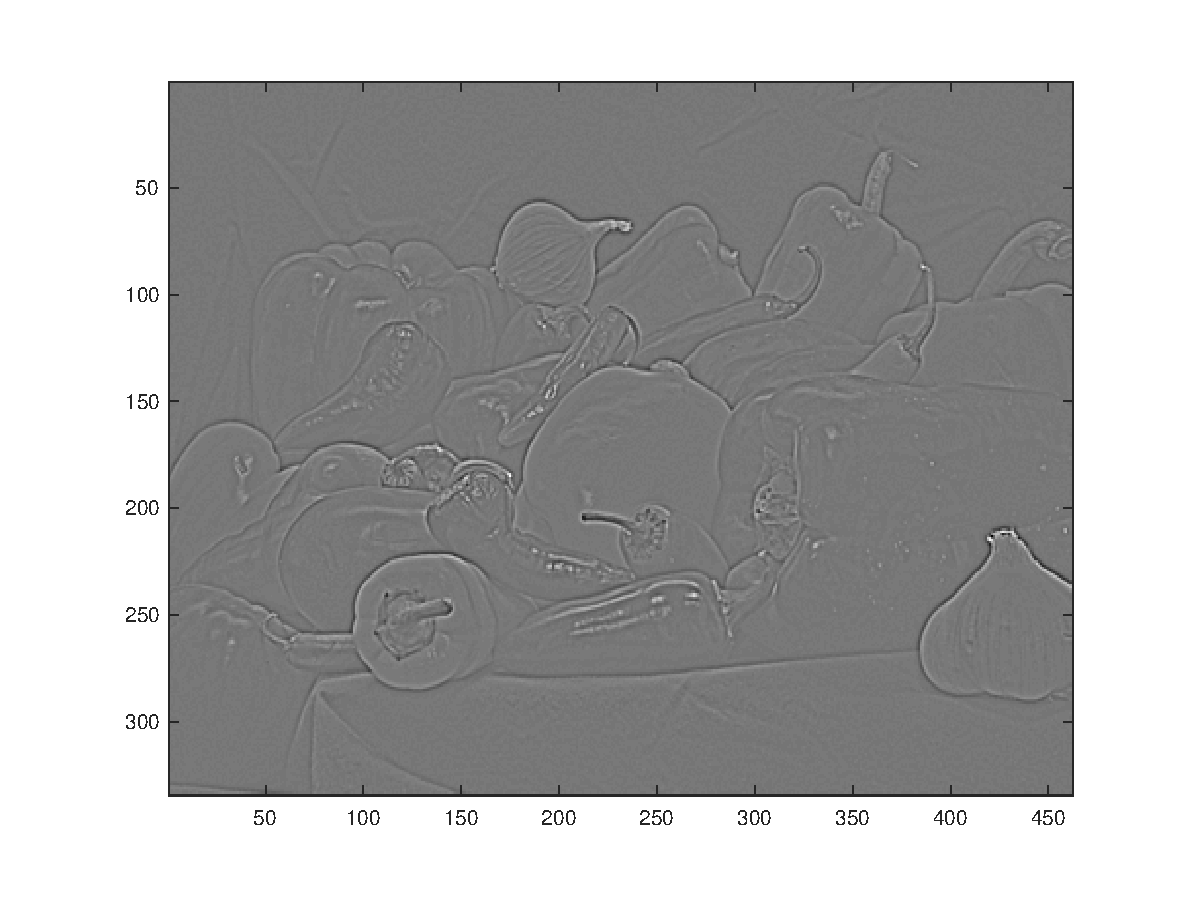
\includegraphics[width=1\textwidth]{peppers_dog3_conv.eps}
\caption{The result of convolving the peppers image with the narrower filter from part E.}
\label{fig:pepper_narrow}
\end{figure}

For the reader, we reproduce our entire code used for this question below before moving on to the next question:
\lstinputlisting{earlyvision.m}

\section{Invariance and Representational Similarity in Deep Neural Networks}

\subsection{AlexNet Filters}

We plot the weights of the AlexNet filters using the code below and show the result in Figure \ref{fig:AlexWeights}. 
\lstinputlisting[firstline=1, lastline=23]{deepnet_invariance.m}

We can see from this that there are several neurons that respond to oriented lines/bars as well as edges. These oriented bars are of various widths. There are also a few neurons that respond to circular edges in its receptive field (though these edges do not have to lie entirely within the receptive field). 

\begin{figure}[ht!]
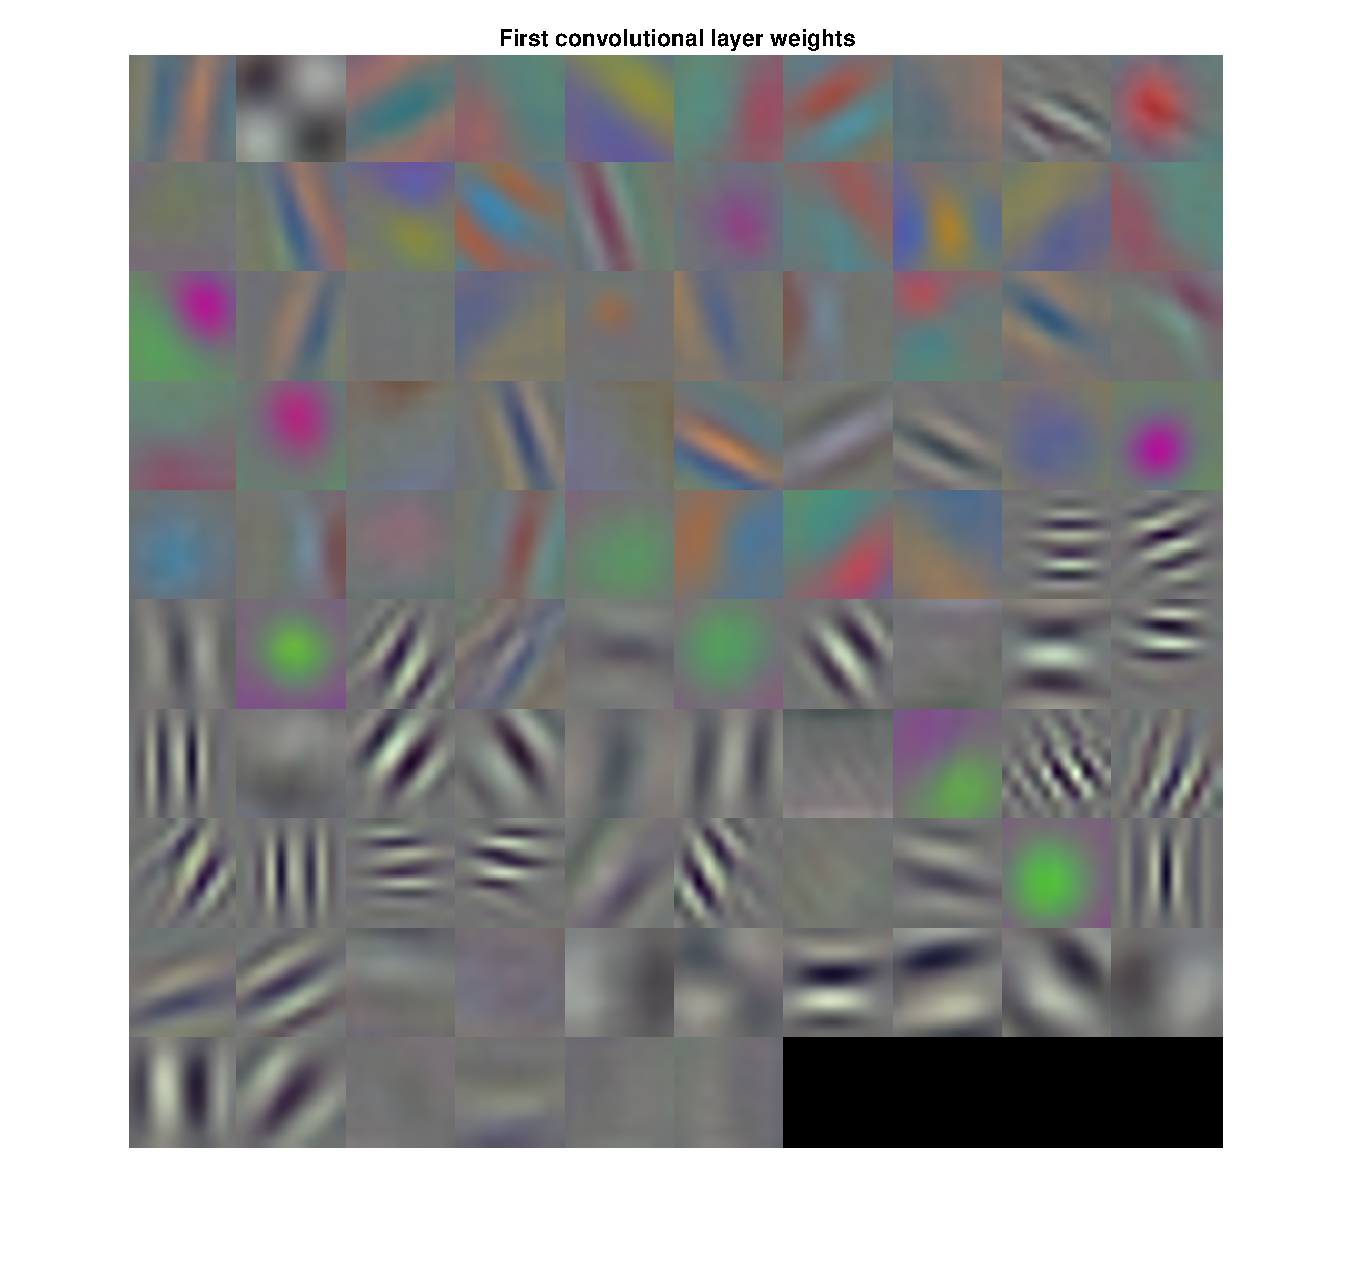
\includegraphics[width=1\textwidth]{alex_weights.eps}
\caption{The weights of the first convolutional layer of AlexNet.}
\label{fig:AlexWeights}
\end{figure}

\subsection{Applying the Network to Peppers}

We apply the network to the peppers image with the following code:
\lstinputlisting[firstline=24, lastline=29]{deepnet_invariance.m}

\begin{figure}[ht!]
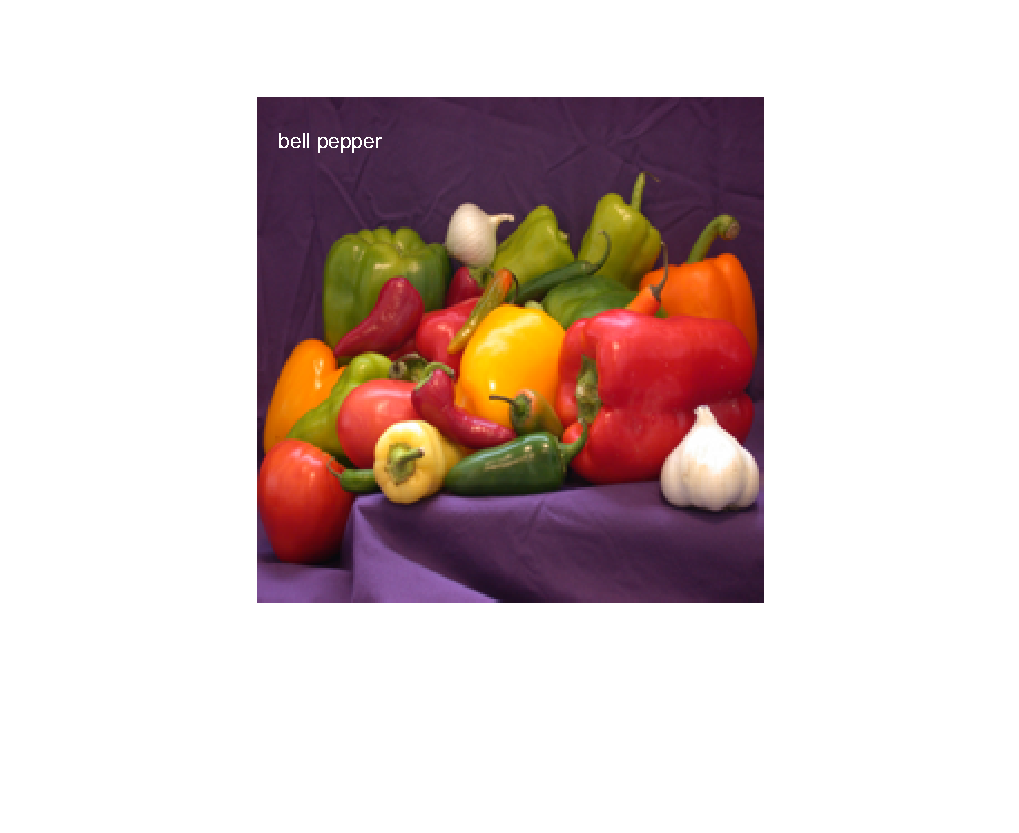
\includegraphics[width=1\textwidth]{pepper_classify.eps}
\caption{The result of running an image through AlexNet.}
\label{fig:pepClassified}
\end{figure}

This produces Figure \ref{fig:pepClassified}, which we can see correctly classifies the image as a bell pepper (to be fair, there are multiple bell peppers within the image, but the network wasn't trained to report how many peppers there are). We then plot the activity of the neurons in the first convolution layer using the following code:
\lstinputlisting[firstline=31, lastline=52]{deepnet_invariance.m}

From our investigation of the neurons in this layer, the activity of filters 3, 10, and 59 are of interest and are plotted in Figures \ref{fig:f3}, \ref{fig:f10}, and \ref{fig:f59}. From these figures, we can see that filter 3 is selective for the rough outlines of the peppers (it is certainly not 100\% accurate or does so in extreme detail). Conversely, filter 10 is selectively for the bodies of the peppers, particularly those that are warm-colored. Filter 59 appears to also be selective for edges or outlines, as can be seen from the fact that it picks up the edge of the table on which the peppers lay very well. 
\begin{figure}[ht!]
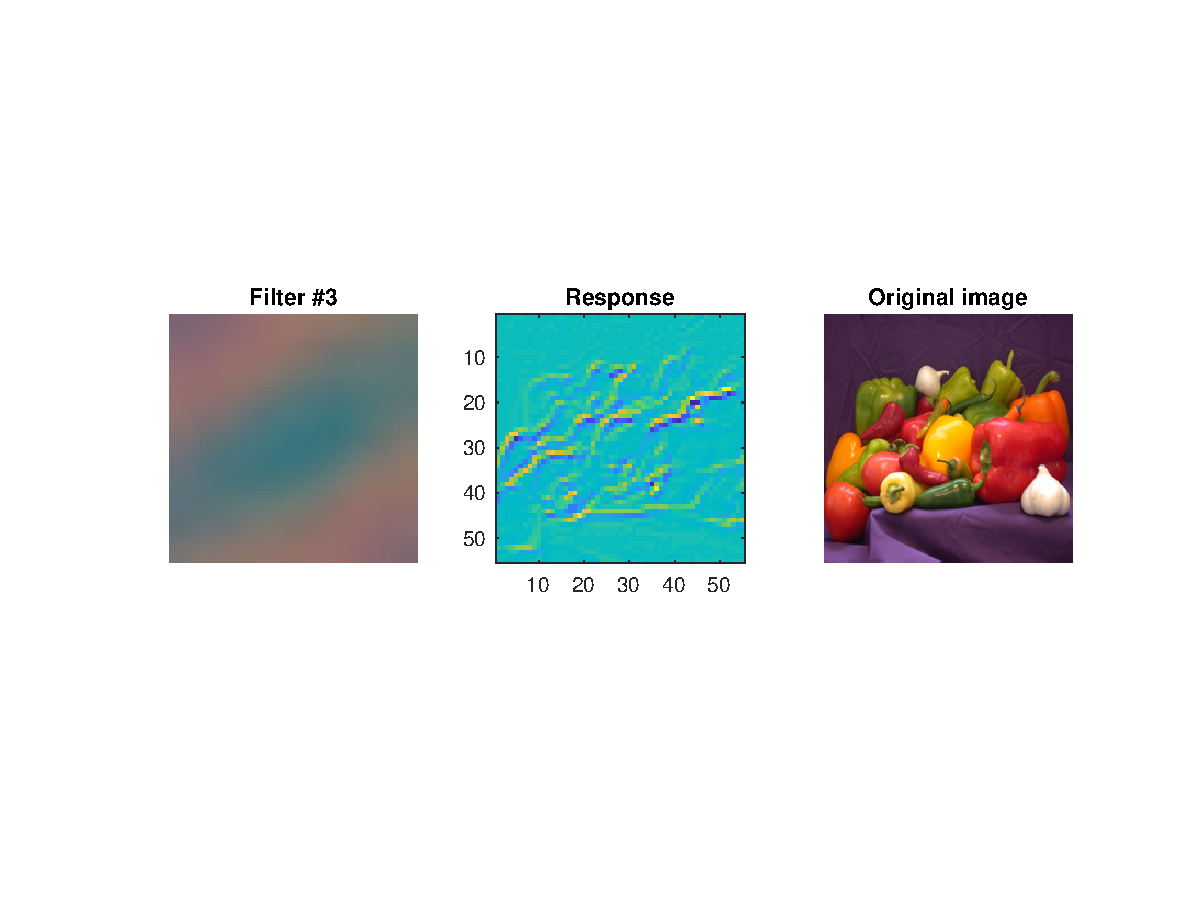
\includegraphics[width=1\textwidth]{filter3.eps}
\caption{The activity of filter 3 in the first convolutional layer when running the pepper image through AlexNet.}
\label{fig:f3}
\end{figure}

\begin{figure}[ht!]
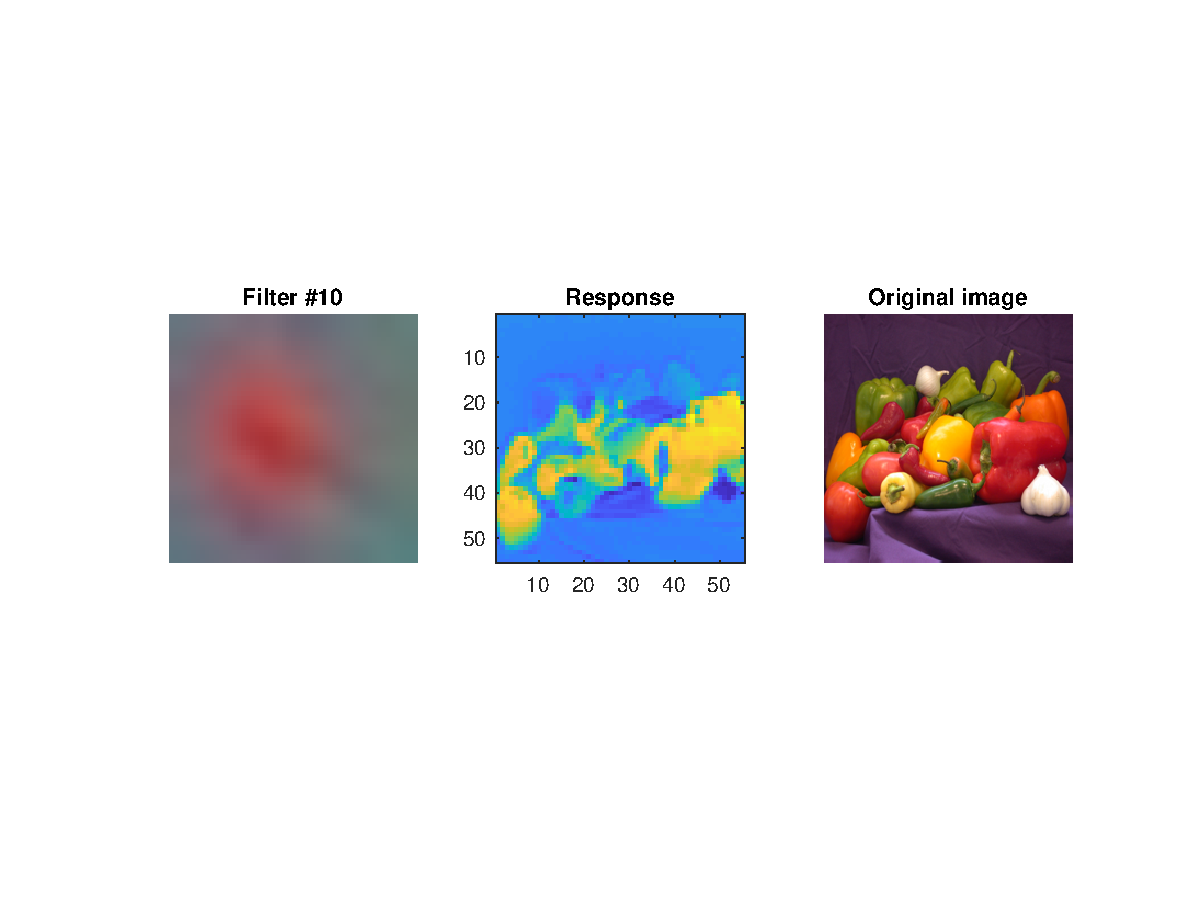
\includegraphics[width=1\textwidth]{filter10.eps}
\caption{The activity of filter 10 in the first convolutional layer when running the pepper image through AlexNet.}
\label{fig:f10}
\end{figure}

\begin{figure}[ht!]
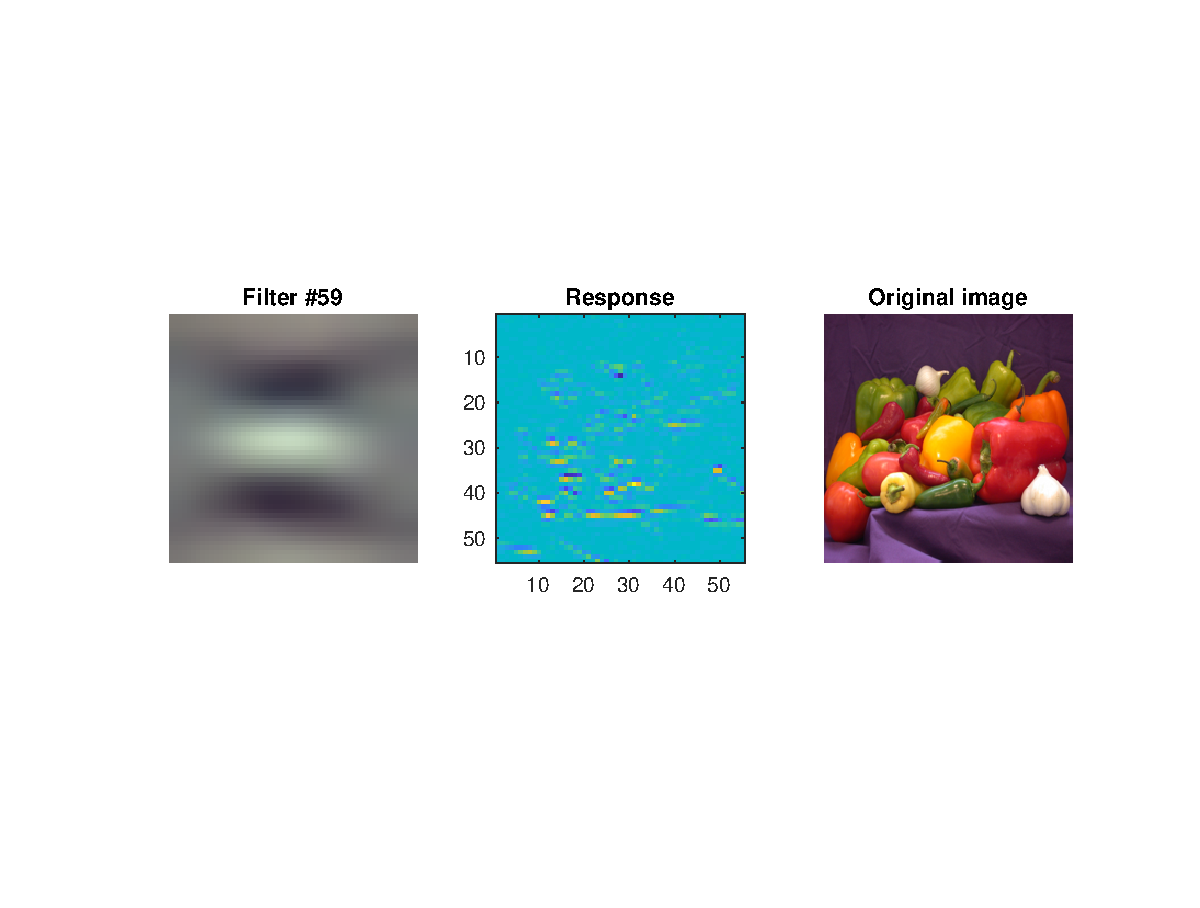
\includegraphics[width=1\textwidth]{filter59.eps}
\caption{The activity of filter 59 in the first convolutional layer when running the pepper image through AlexNet.}
\label{fig:f59}
\end{figure}

\subsection{Translation Invariance of AlexNet}

We plot the correlation between activations for the original image and the image translated to the right using the following code:
\lstinputlisting[firstline=54, lastline=84]{deepnet_invariance.m}
This produces Figure \ref{fig:netTrans}, which shows us that higher layers of the network are more invariant to translation, evident by their higher correlation with the activations produced by the original image. Further, we can see that pooling layers are more invariant than convolution layers as at every stage investigated here, the pooling layer had a higher invariance than the convolution layer. Further, in some cases, the convolution layer seemed to decrease translation invariance overall, as can be seen by the fact that the first convolutional layer had a lower correlation than the correlation between the translated image and the original image (i.e. the data layer).

\begin{figure}[ht!]
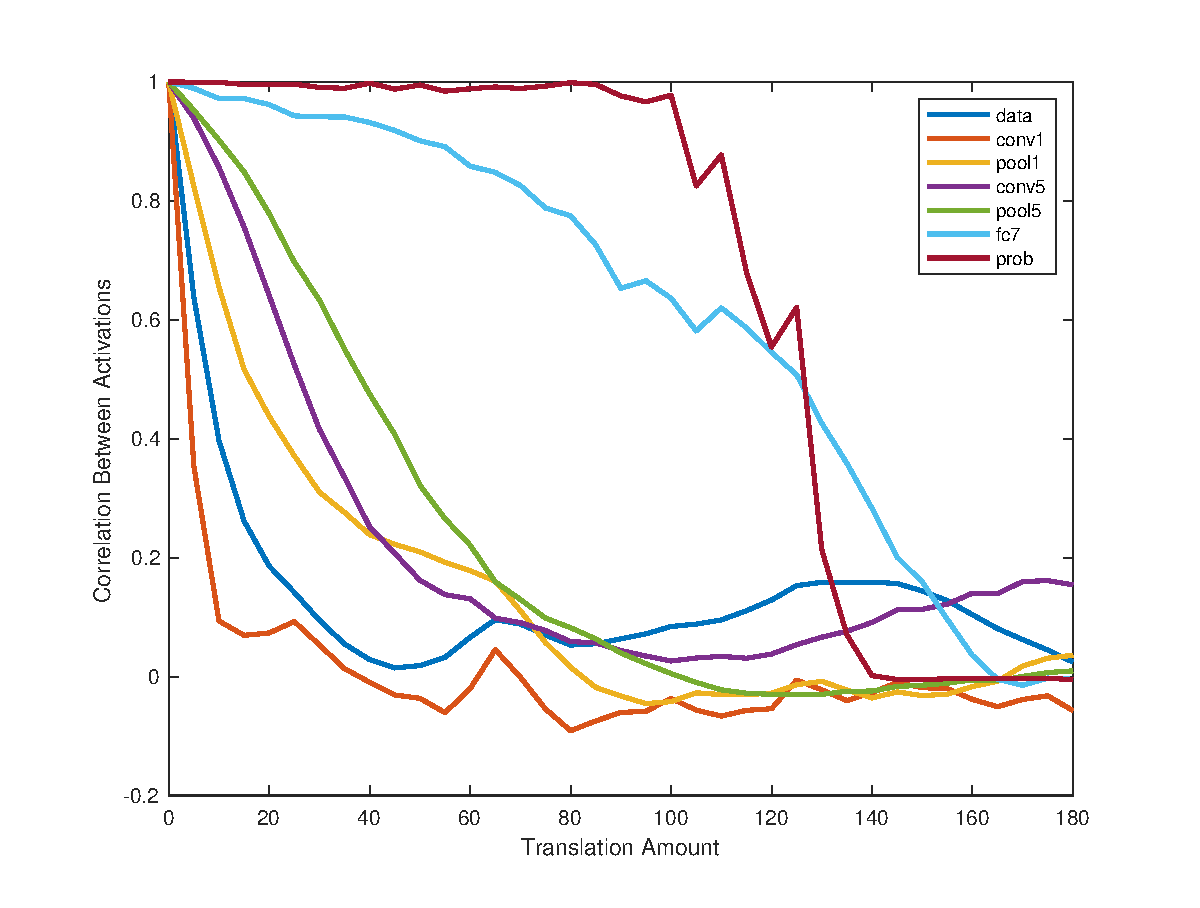
\includegraphics[width=1\textwidth]{trans_invar.eps}
\caption{The translation invariance of several layers in AlexNet using an image of a German Shepherd.}
\label{fig:netTrans}
\end{figure}

\subsection{Rotation Invariance of AlexNet}

We plot the correlation between activations for the original image and the image rotated using the following code:
\lstinputlisting[firstline=86, lastline=111]{deepnet_invariance.m}
This produces Figure \ref{fig:netRot}, which shows us that AlexNet begins to misclassify the image around an angle of 30 degrees (as evident by the probability layer). Thus, it is clear that AlexNet is more resistant to translation than rotation.

\begin{figure}[ht!]
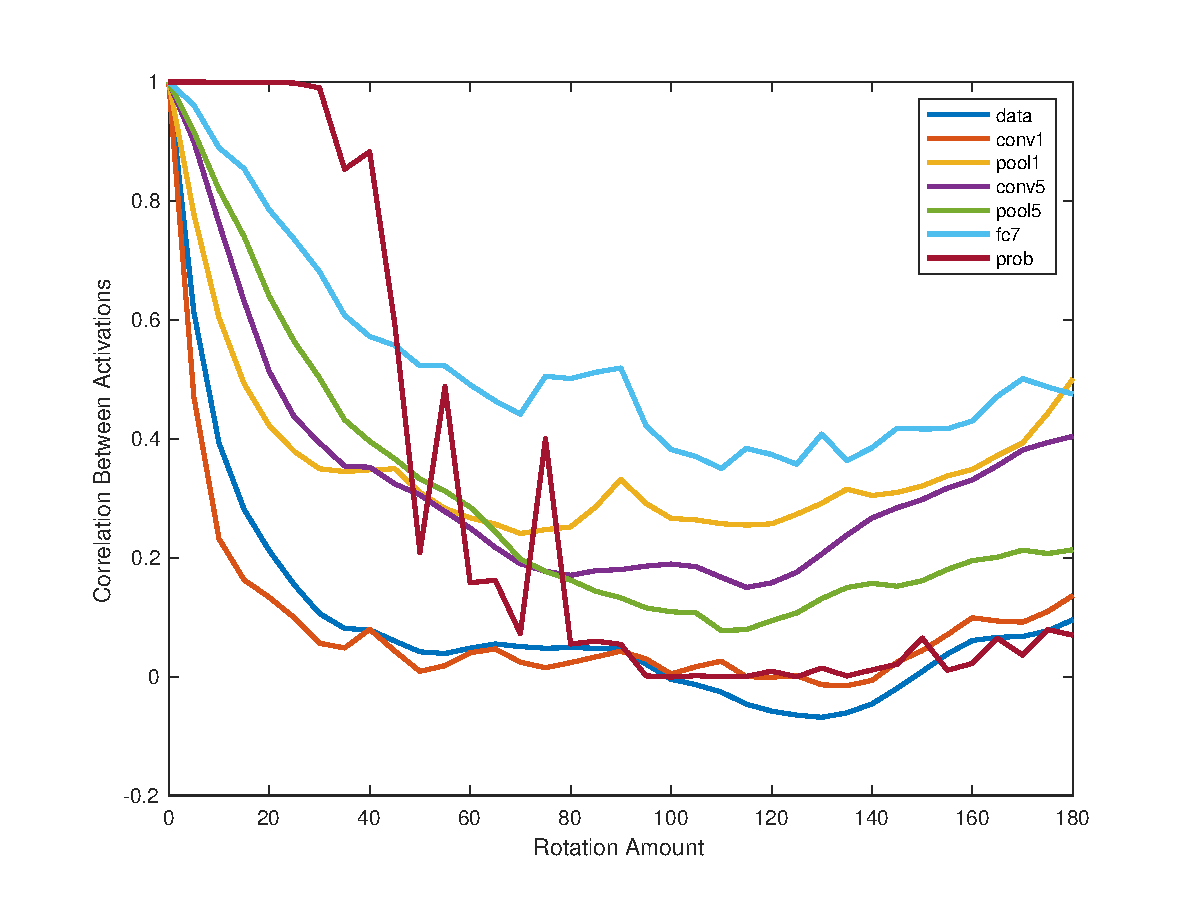
\includegraphics[width=1\textwidth]{rot_invar.eps}
\caption{The rotation invariance of several layers in AlexNet using an image of a German Shepherd.}
\label{fig:netRot}
\end{figure}

\subsection{Correlation between RDM of AlexNet and real neural activity}

We computed the RDM for AlexNet and the correlation between the AlexNet RDMs and the experimental RDMs using the following code:
\lstinputlisting[firstline=113, lastline=144]{deepnet_invariance.m}
We ran this twice to look at how AlexNet compares both to the monkey recording (Figure \ref{fig:corrMonkey}) and the human fMRI data (Figure \ref{fig:corrHuman}). We can see from these figures that the RDMs of intermediate layers in AlexNet are more similar to the experimental RDMs than the raw data. Indeed, for both datasets, the relu5 (the 5th convolutional layer after the ReLU activation function has been applied) best matched the experimental RDMs (as evident by it having the highest correlation).

\begin{figure}[ht!]
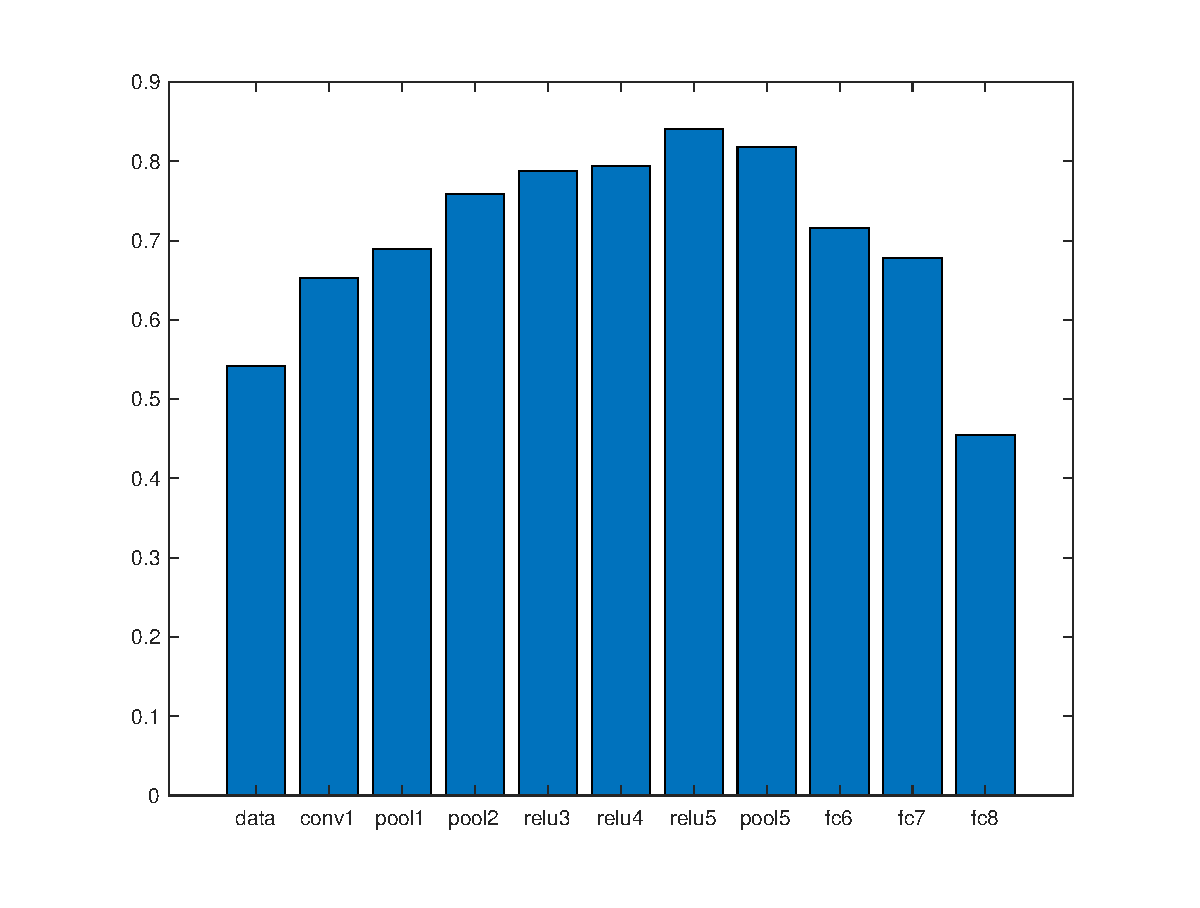
\includegraphics[width=1\textwidth]{corrMonkey.eps}
\caption{The correlation coefficient between the RDM of various layers in AlexNet and electrode recordings in monkeys.}
\label{fig:corrMonkey}
\end{figure}

\begin{figure}[ht!]
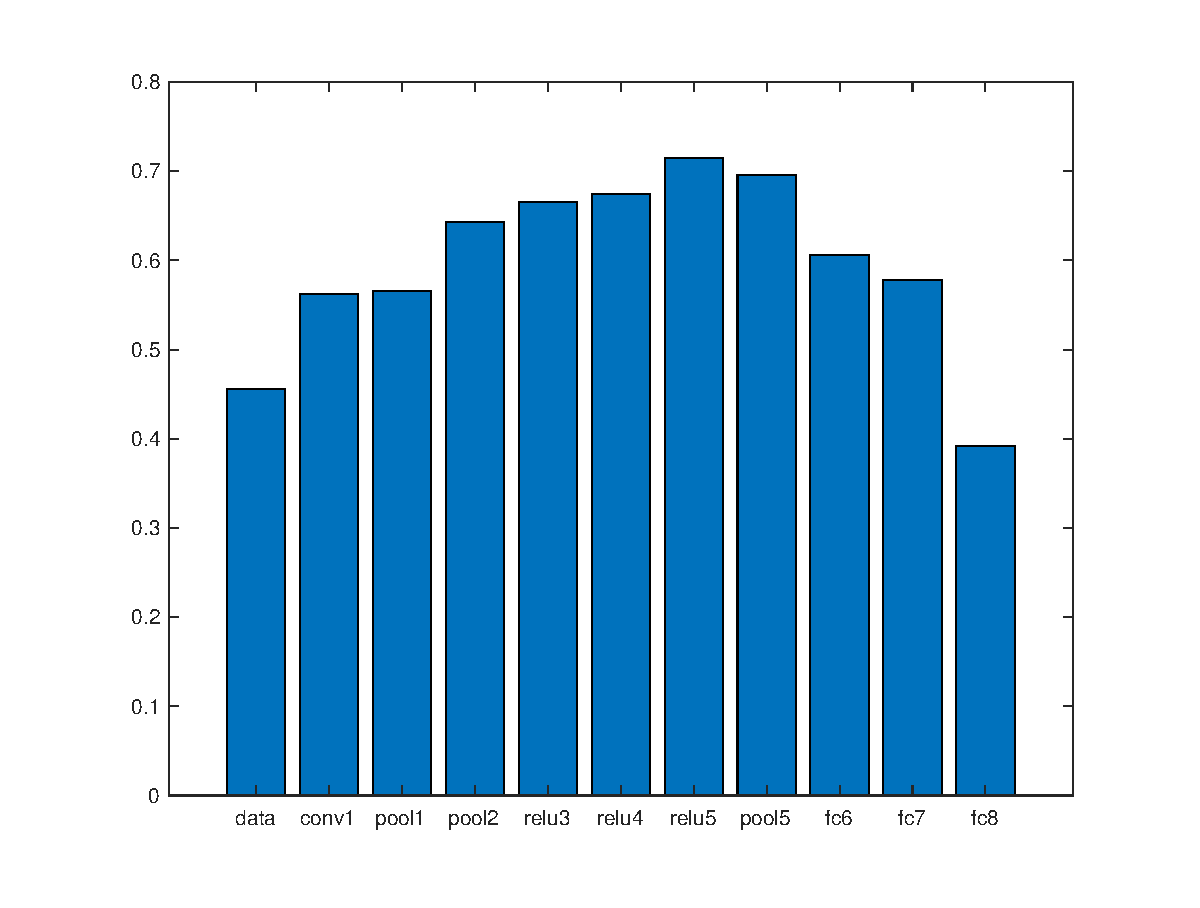
\includegraphics[width=1\textwidth]{corrHuman.eps}
\caption{The correlation coefficient between the RDM of various layers in AlexNet and fMRI recordings in humans.}
\label{fig:corr:Human}
\end{figure}

\section{Back Propagation and Deep Learning}

\subsection{Gradient Descent}

We implement gradient descent using the following code:
\lstinputlisting{backprop.m}

This produces Figure \ref{fig:netMetrics}, which shows the change in loss and accuracy on both the training and test data over time.

\begin{figure}[ht!]
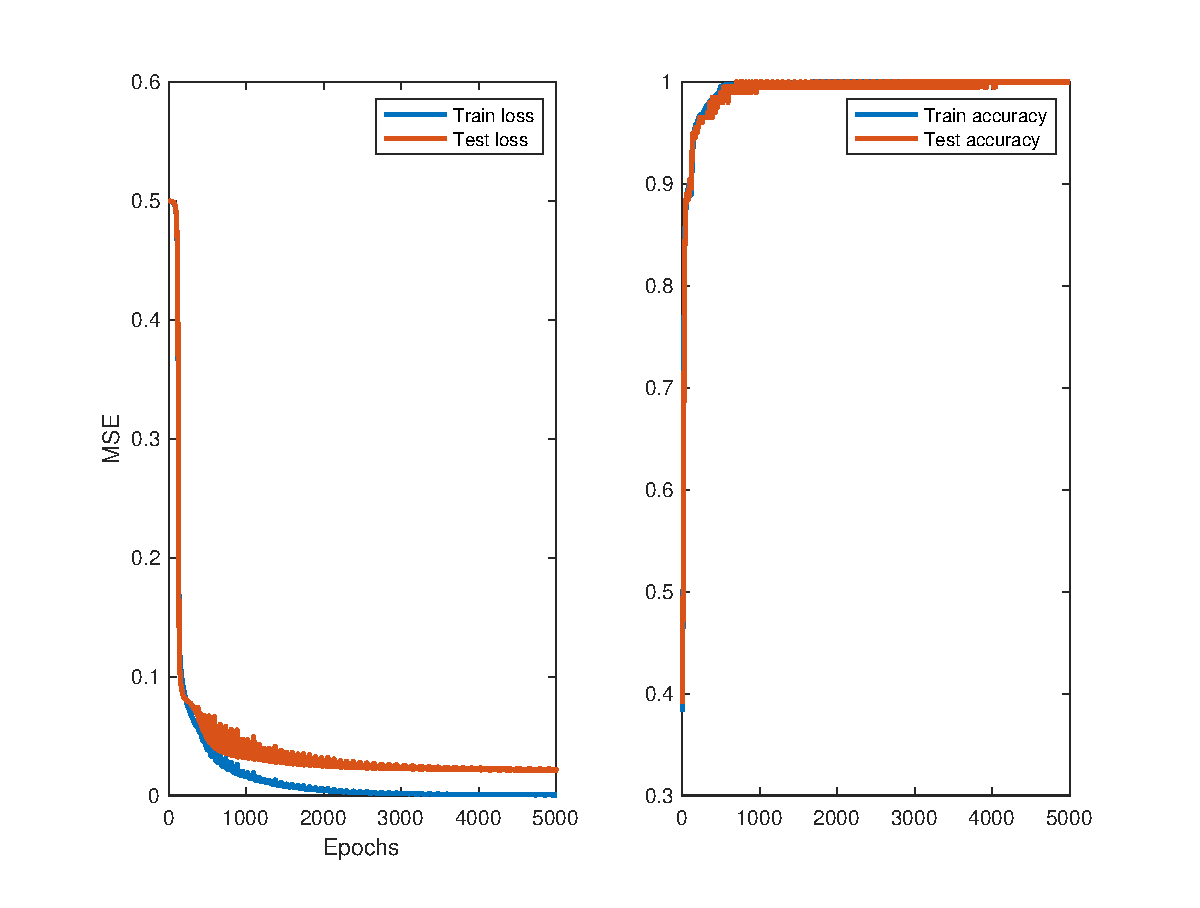
\includegraphics[width=1\textwidth]{netMetrics.eps}
\caption{The loss and accuracy of both training and test data for a neural net trained on a subset of MNIST data.}
\label{fig:netMetrics}
\end{figure}

\subsection{Reflections on the Neural Net}

We can see from the loss and accuracy graphs that this neural net performs quite well on both training data and test data with an accuracy of 100\% by the end of training. Because the model performed 100\% accuracy on the test data, we can conclude that there was no overfitting, so there is no need to stop training early, though it appears we could stop at around 4000 steps as the accuracy peaked at 100\% near there and maintained that level.

\subsection{Larger Weight Scale}

We ran the code above again changing only \lstinline{weight_scale = .1;}, and plot the results in Figure \ref{fig:netMetrics2}. We can see from this that it does not substantially impact the training accuracy, but it does result in a small decrease of the test accuracy to about 99\%. Stopping training early in this case, however, would not help the test accuracy as the larger weight variance removed any oscillations in the loss and accuracy that we saw before and resulted in a slow but steady increase of the accuracy that resulted in an asymptote. Thus, it seems that the smaller weight variance and not this larger weight variance might be better for the purposes of generalization based on our findings. 

\begin{figure}[ht!]
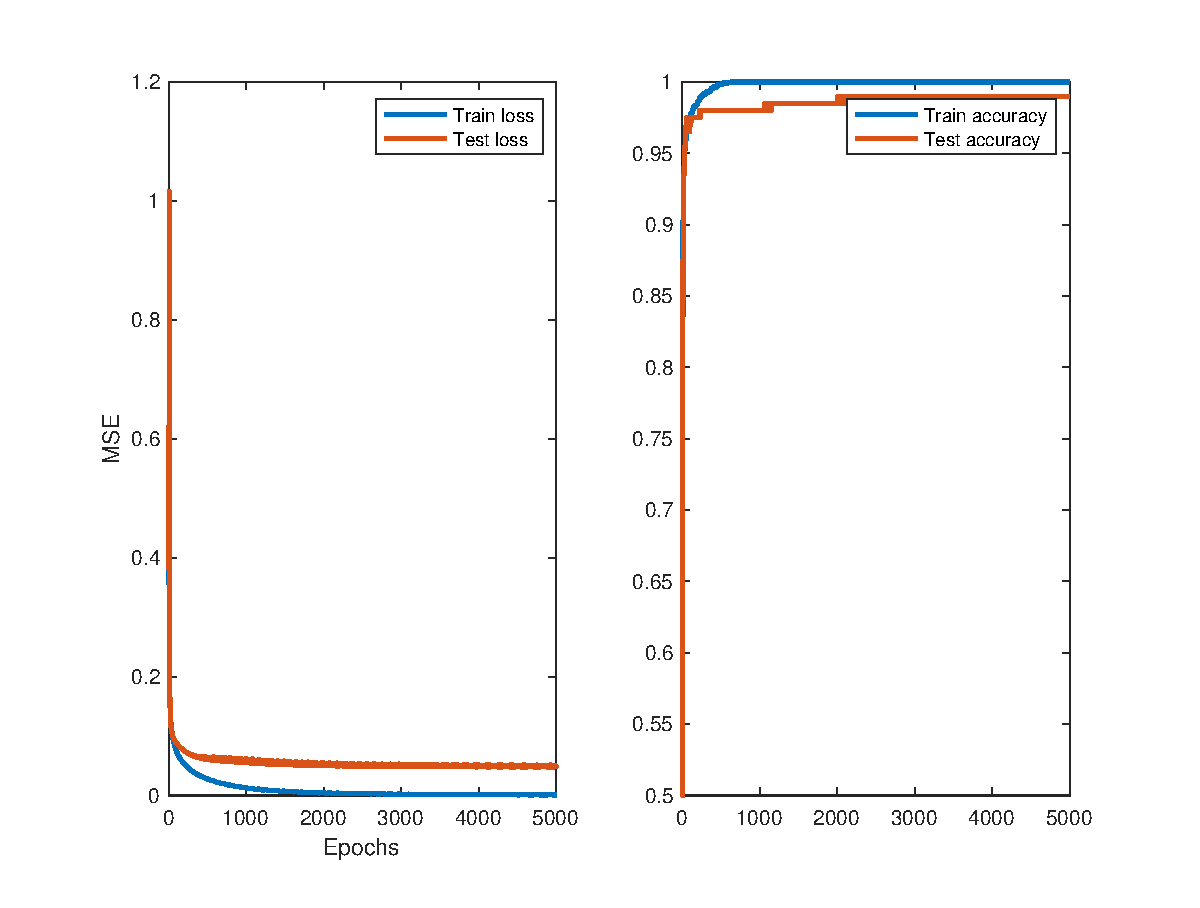
\includegraphics[width=1\textwidth]{netMetrics2.eps}
\caption{The loss and accuracy of both training and test data for a neural net trained on a subset of MNIST data with a larger weight scale of 0.1.}
\label{fig:netMetrics2}
\end{figure}

\end{document}
